\documentclass[letterpaper, 12pt]{article}
\usepackage[margin=1in]{geometry}
\usepackage{graphicx}
\usepackage{listings}
\usepackage{amsmath}
\graphicspath{{images/}{../Template/images/}}
\lstset{language=[Motorola68k]assembler,basicstyle=\ttfamily,frame=single}

\newcommand{\hwnumber}{Lab 5}
\newcommand{\duedate}{October 27th, 2015}

\newcommand{\capper}{\begin{flushright}Aviles, Jean-Ralph \\ EEL3744 \\ Section 1539 \\ \duedate{} \\ \hwnumber{}\end{flushright}}

\begin{document}
\capper{}
\section*{Questions}
\begin{enumerate}
  \item List the XMEGA's USART registers used in your programs and briefly describe their functions.
  \begin{enumerate}
    \item CTRLA \\
      \hspace*{8pt} Determines whether interrupts will fire for specific USART events.
    \item CTRLB \\
      \hspace*{8pt} Enables Tx and Rx pins for USART
    \item CTRLC \\
      \hspace*{8pt} Sets the serial's parity, stop bits, character length, etc.
    \item BAUDCTRLA \\
      \hspace*{8pt} Lower 8 bits of BSEL
    \item BAUDCTRLAB \\
      \hspace*{8pt} Upper 8 bits of BSEL and BSCALE
  \end{enumerate}
  \item What is the difference between serial and parallel communication? \\
    \hspace*{8pt} Serial communication transfers information -- bits -- one at a time, while a parallel communication transfers all bits at the same time.
  \item List the number of bounces from part A of this lab. How long (in ms) is your delay routine for debouncing? \\
    \hspace*{8pt} I was getting about 2-3 bounces per flip. However I set my delay to 1ms because my finger touching the switch would cause more bounces for a longer period of time.
  \item What is the maximum possible baud you can use \textbf{for asyncronous communication} if your board runs at 2Mhz? Support your answer with the values you would place in any special registers that are needed. \\
    \hspace*{8pt} Using double clock speed mode, our baud rate is bounded by the equation\ldots \[ f_{baud} \leq \frac{f_{per}}{8} \] Plugging in our clock rate of 2MHz, we get a maximum baud rate of \textbf{250 kbps}.
\end{enumerate}
\section*{Problems Encountered}
I tried using GNU screen as my tty, but I couldn't get it configured correctly.
\section*{Future Work/Applications}
Serial can be used to communicate between our AVR and our laptops or even other microcontrollers. The possibilities with serial communication are endless.
\section*{Appendix}
\subsection*{Part A}
\begin{enumerate}
    \item How many times did your interrupt service routine get called when you pulled the switch? \\
      \hspace*{8pt} About 2-3 times per flip.
\end{enumerate}
\subsubsection*{Switch Bouncing}
\begin{center}
  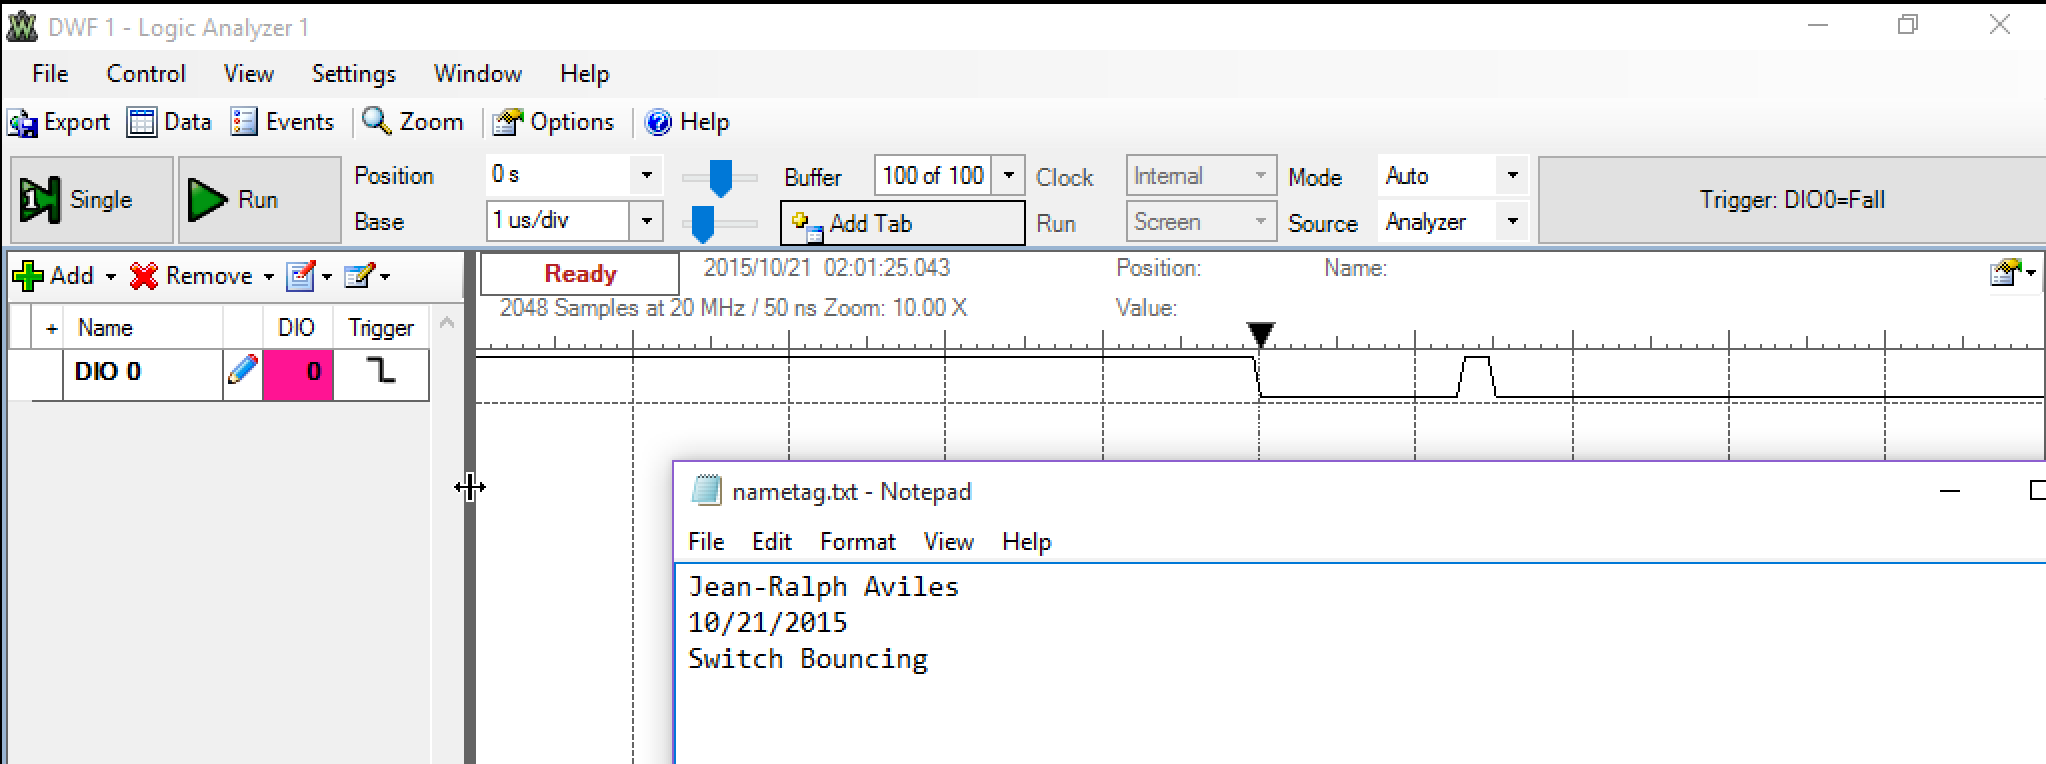
\includegraphics[scale=0.5]{bouncing}
\end{center}
\subsection*{Part B}
\begin{enumerate}
    \item What pins on PORTD are used for USART0?
      \begin{enumerate}
          \item Pin1 - XCK0
          \item Pin2 - RXD0
          \item Pin3 - TXD0
      \end{enumerate}
    \item USART Configurations \\
    CPU\_Clock = 2MHz \\
    BSCALE = -7 \\
    F$_{baud}$ = 14.4kHz \\
    \( BSEL = \frac{1}{2^{BSCALE}}\left( \frac{CPU\_CLOCK}{16\cdot BAUD -1}\right) = \frac{1}{2^{-7}}\left(\frac{2e6}{230400}-1\right) = 983.\overline{11} \)
\end{enumerate}
\section*{Pseudocode/Flowcharts}
\subsection*{Part A}
\subsubsection*{Counter Pseudocode}
\lstinputlisting{code/Lab5_counter.ps}
\subsection*{Part C}
\subsubsection*{Out Char Pseudocode}
\lstinputlisting{code/Lab5_outchar.ps}
\subsubsection*{Out String Pseudocode}
\lstinputlisting{code/Lab5_outstring.ps}
\subsubsection*{In Char Pseudocode}
\lstinputlisting{code/Lab5_inchar.ps}
\subsection*{Part D}
\subsubsection*{PartD Pseudocode}
\lstinputlisting{code/Lab5_D.ps}
\section*{Programs}
\subsection*{Part A}
\subsubsection*{Counter Assembly}
\lstinputlisting{code/Lab5_counter.asm}
\subsection*{Part C}
\lstinputlisting{code/Lab5_C.asm}
\subsection*{Part D}
\lstinputlisting{code/Lab5_D.asm}
\end{document}
